\documentclass{patmorin}
\usepackage{pat}
\usepackage{amsopn}

\DeclareMathOperator{\obs}{obs}

\title{On Obstacle Numbers}
\author{Bellairs Geometry and Graphs 2013}

\begin{document}
\maketitle

\begin{abstract}
The obstacle number of a graph is an interesting new graph parameter
introduced by Alpert, Koch, and Laison (2010).  Pach \etal\ (2012)
show that there exist graphs with $n$ vertices having obstacle
number in $\Omega(n/\log n)$. In this paper we up this lower bound to
$\Omega(n/(\log\log n)^2)$
\end{abstract}

\newpage

\section{Introduction}

The obstacle number of a graph is a new graph parameter introduced by
Alpert, Koch, and Laison \cite{alpert.koch.ea:obstacle}.

Let $G=(V,E)$ be a graph, let $\varphi:V\to \R^2$ be a one-to-one mapping
of the vertices of $G$ onto $\R^2$, and let $S$ be a set of connected
subsets of $\R^2$.  The pair $(\varphi,S)$ is an \emph{obstacle
representation} of $G$ if and only if, for every pair of vertices
$u,w\in V$, the edge $\{u,w\}\in E$ if and only if the open line segment
with endpoints $\varphi(u)$ and $\varphi(w)$ does not intersect any
\emph{obstacle} in $S$.  The \emph{obstacle number} of a graph $G$,
denoted by $\obs(G)$, is the minimum number of obstacles in any obstacle
representation of $G$.

\figref{fivebyfive} shows a surprising example of an obstacle
representation of the $5\times 5$ grid graph that uses only one obstacle.
Since at least one obstacle is necessary to represent any graph other
than a complete graph, this proves that the $5\times 5$ grid graph has
obstacle number 1.

\begin{figure}
  \begin{center}
    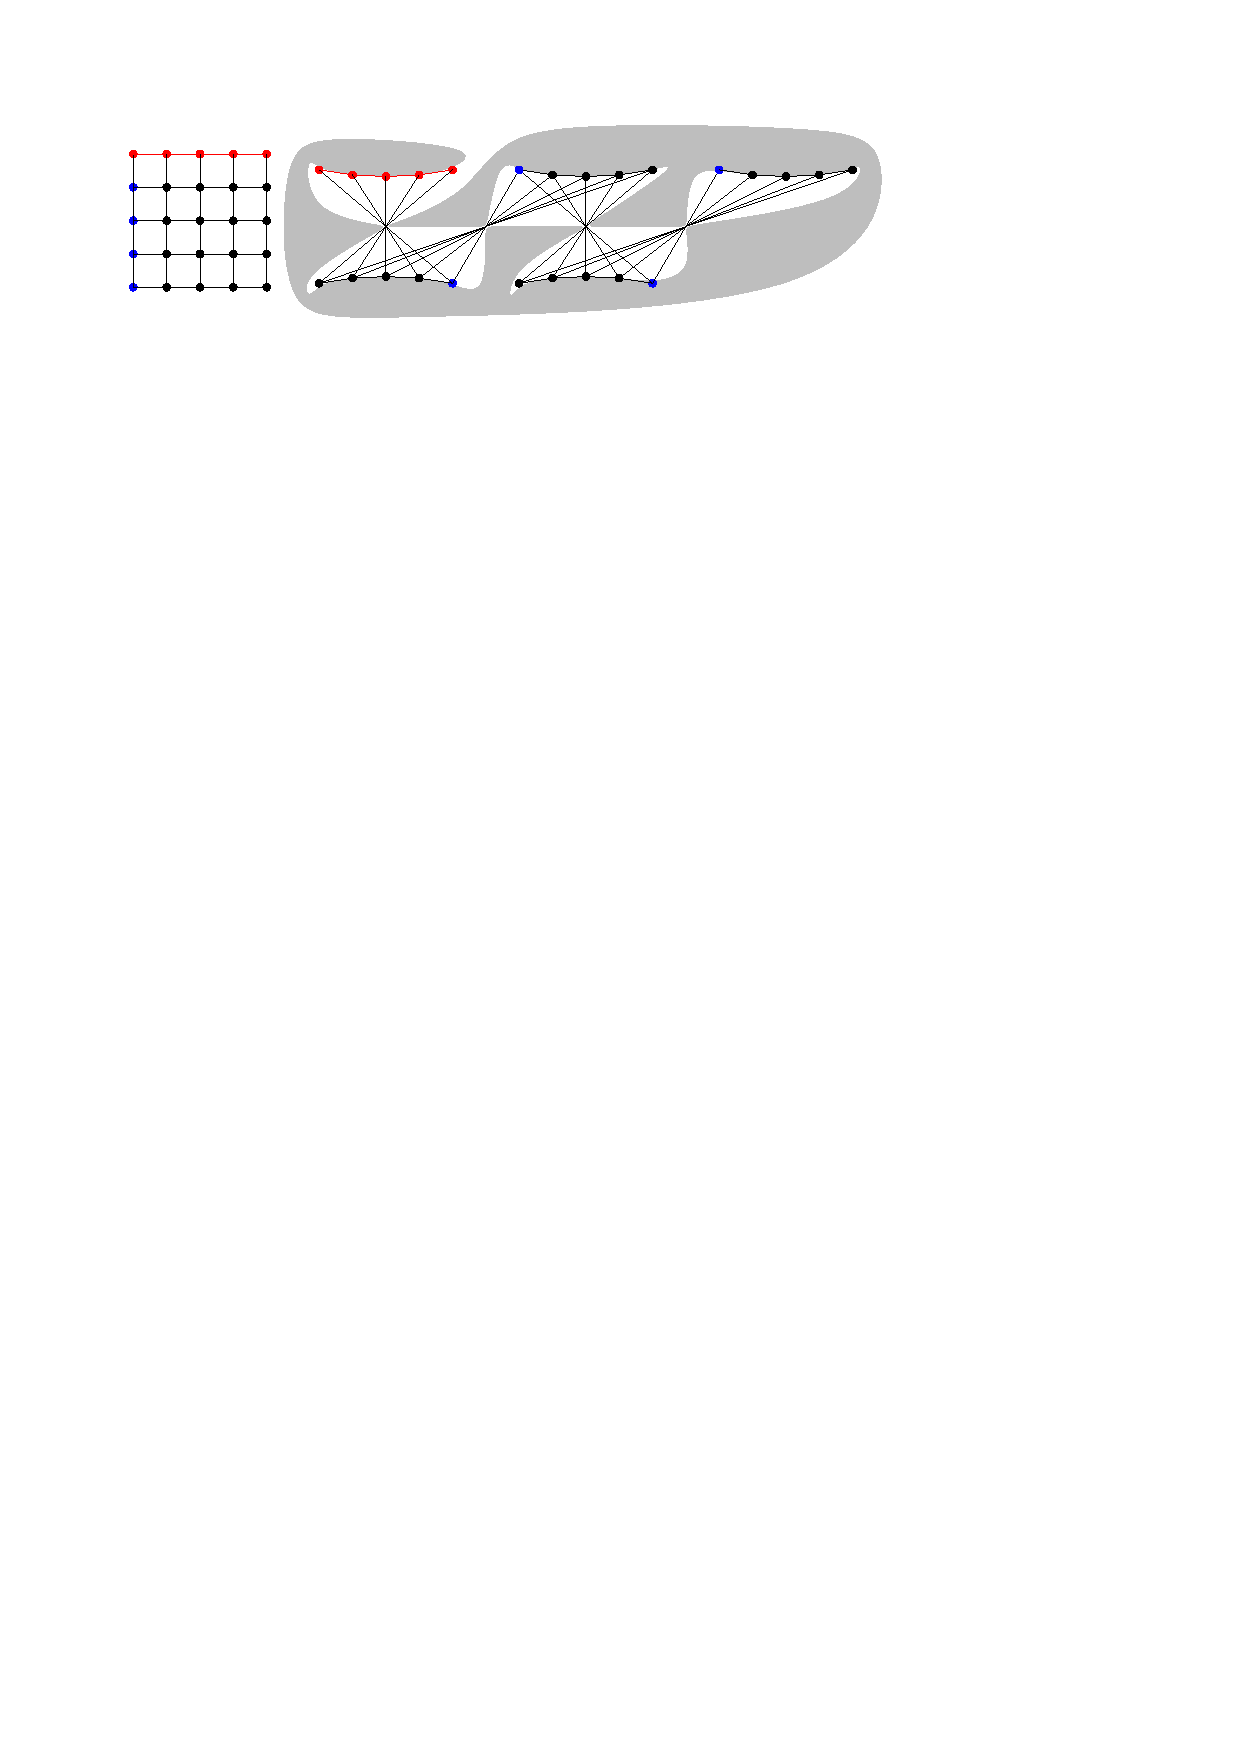
\includegraphics{fivebyfive}
  \end{center}  
  \caption{The $5\times 5$ grid graph has obstacle number 1.}
  \figlabel{fivebyfive}
\end{figure}

Since their introduction, obstacle numbers have generated a significant
amount of research interest \ldots \note{Literature review goes here.}

A fundamental---and far from answered---question about obstacle numbers
is that of determining the \emph{worst-case obstacle number},
\[
    w(n) = \max \{\obs(G) :\mbox{$G$ is a graph with $n$ vertices}\}
    \enspace ,
\] 
of a graph with $n$ vertices.

The worst-case obstacle number is obviously upper-bounded by
$\binom{n}{2}\in O(n^2)$ since, by drawing the vertices of a graph
 on a point set in sufficiently general position, one can place
a small obstacle---even a single point---on the mid-point of each
line segment $uw$ for every pair of vertices $u$ and $w$ such that
$uw\not\in E$.  If the vertices are in sufficiently general position,
then, for each pair of vertices $u$ and $w$, the line segment $uw$ will
intersect an obstacle if and only if $uw\not\in E$.  No upper-bound
asymptotically better than $O(n^2)$ is known.

On the lower-bound side, Alpert \etal\ initially show that the worst-case
obstacle number is $\omega_n(1)$.\footnote{Alpert \etal's
lower-bound uses the Erd\"os-Szekeres convex $n$-gon theorem and shows
the existence of an $n$-vertex graph $G$ with $\obs(G)\ge \sqrt{\log
n/\log\log n}$.} Pach \etal\ \cite{pach.x.y} showed that there exist
graphs on $n$ vertices with obstacle number $\Omega(n/\log^2 n)$.
Mukkamala \etal\ \cite{mukkamala.pach.ea:lower} later upped this bound
to $\Omega(n/\log n)$.  In the current paper, we up the lower-bound
again by proving the following theorem:
\begin{thm}\thmlabel{main}
  For every integer $n>0$, there exists a graph $G$ with $n$ vertices
  and $\obs(G)\in\Omega(n/(\log\log n)^2)$.
\end{thm}

\section{The Proof}

We make use of the following theorem, due to Mukkamala, Pach, and
P\'alv\"olgyi about the number of $n$ vertex graphs with obstacle number
at most $h$:
\begin{thm}[Mukkamala, Pach, and P\'alv\"olgyi 2012]\thmlabel{pach-gang}
  For any $h\ge 1$, the number of graphs having $m$ vertices and
  obstacle number at most $h$ is at most $2^{O(hn\log^2 n)}$.
\end{thm}

The following lemma shows that, for random graphs, a fixed point
set and fixed embedding is \emph{very} unlikely to yield an obstacle
representation with few obstacles.

\begin{lem}\lemlabel{fixed}
  Let $G=(V,E)$ be an Erd\"os-Renyi random graph $G_{n,\frac{1}{2}}$,
  let $P\subset\R^2$ be a set of $n$ points in general position, let
  $\varphi:V\rightarrow P$ be a bijection between $V$ and $P$ that is
  independent of the choices of edges in $G$, and let $(\varphi, S)$ be
  an obstacle representation of $G$ using the minimum number of obstacles
  (subject to $G$ and $\varphi$).  Then, for any constant $c>0$,
  \[
     \Pr\{|S| \in \Omega(n/(\log\log n)^2) \ge 1-e^{-\Omega(cn\log n)}  \enspace .
  \] 
\end{lem}

\begin{proof}
Fix some integer $k$ to be specified later and first consider some
arbitrary subset $P'\subset P$ of $k$ points and let $G'=(V',E')$
be the subgraph of $G$ induced by the set $V'=\{\varphi^{-1}(x):x\in
P'\}$ of vertices that are mapped by $\varphi$ to $P'$.  Applying
\thmref{pach-gang} with $n=k$ and $h=\alpha k/\log^2 k$, we obtain
\begin{equation}
     \Pr\{\obs(G') \le \alpha k/\log^2 k\} 
       \le \frac{2^{O(\alpha n^2)}}{2^{\binom{k}{2}}}
       = 2^{-\Omega(k^2)} \enspace , \eqlabel{g1}
\end{equation}
for a sufficiently small constant $\alpha > 0$.  Note that, if
$\obs(G')\ge h$, then, in the obstacle representation of $(\varphi,S)$,
there must be at least $h-1$ obstacles of $S$ that are contained in the
convex hull of $P'$.\note{Room for improvement here. \thmref{pach-gang}
is way stronger than we need. We're given the embedding, so there should
be way fewer graphs we can represent with $h$ obstacles.}

Without loss of generality assume that no two points in $P$ have the
same x-coordinate and denote the points in $P$ by $x_0,\ldots,x_{n-1}$
by increasing order of x-coordinate.  Let $m=\lfloor n/k\rfloor$ and
consider the point sets $P'_0,\ldots,P'_{m-1}$, where
\[ 
  P_i'=\{x_{ik},x_{ik+1},\ldots,x_{(ik+k-1}\} \enspace .
\]  
That is, $P_0',\ldots,P_{m-1}'$ are determined by vertical slabs,
$s_0,\ldots,s_{m-1}$ that each contain $k$ points.  \Eqref{g1} shows
that, with probability at least $1-2^{-\Omega(k^2)}$, the obstacle
number of the subgraph that maps to $P'_i$ is $\Omega(k/\log^2 k)$.
If this occurs, then $S$ has $\Omega(k/\log^2 k)$ obstacles that are
completely contained in $s_i$.  These obstacles are therefore disjoint
from any other obstacles contained in any other $s_j$, $j\neq i$.

We are proving a lower bound on the number of obstacles, so we are worried
about the case where the number of slabs that do \emph{not} completely
contain $\alpha k/\log^2 k$ obstacles exceeds $m/2$.  The number of
slabs, $M$, not containing $\alpha k/\log^2 k$ obstacles is dominated
by a binomial$(m,2^{-\Omega(k^2)})$ random variable.  Using Chernoff's
bound on the tail of a binomial random
variable,\footnote{%
  Chernoff's Bound: For any binomial$(m,p)$ random variable, $B$,
  any $\delta>0$ and $\mu=mp$, 
  \[ \Pr\{B\ge (1+\delta)\mu\}
     \le \left(\frac{e^{\delta}}{(1+\delta)^{1+\delta}}\right)^{\mu} 
       \enspace . 
  \]}
we have that
\begin{align*}
  \Pr\{M \ge m/2\} & = \Pr\{M\ge (1+\delta)\mu\}
    & \text{(where $\mu=me^{-ck^2}$ and $\delta=e^{ck^2-1}-1$)} \\
    & \le \left(\frac{e^{\delta}}{(1+\delta)^{1+\delta}}\right)^{\mu} \\
    & = \left(\frac{e^{e^{ck^2}}}{(e^{ck^2-1})^{e^{ck^2-1}}}\right)^{me^{-ck^2}}\\
    & = \left(\frac{e^{e^{ck^2}}}{e^{(ck^2-1)e^{ck^2-1}}}\right)^{me^{-ck^2}}\\
    & = \frac{e^{m}}{e^{m(ck^2-1)e^{ck^2-1}e^{-ck^2}}} \\
    & = \frac{e^{m}}{e^{m(ck^2-1)/2}} \\
    & = e^{-\Omega(mk^2)} \enspace .
\end{align*}
Taking $k=\sqrt{c}\log n$ and recalling that $m=\lfloor n/k\rfloor$, we obtain
the desired result.  In particular,
\[
    |S| \ge \Omega\left(\left(k/\log^2 k\right)\times m \right)
      = \Omega\left(n/\log^2\log n\right)
\]
with probability at least
\[
    1-e^{-\Omega(mk^2)} = 1-e^{-\Omega(cn\log n)} \enspace . \qedhere
\]
\end{proof}

The remainder of the proof of \thmref{main} is just an application of
the probabilistic method.  \lemref{fixed} shows that the probabilitly,
$p$, that a particular embedding of the random graph $G$ is able to
yield an obstacle representation with $o(n/(\log\log n)^2)$ obstacles is
extremely small.  Let $N$ be the total number of possible embeddings
of $G$.  Then the union bound shows that $p N$ is an upper-bound on the
probability that there exists any embedding of $G$ that yields an obstacle
representation using $o(n/(\log\log n)^2)$ obstacles.  If $pN <1$, this
implies that, with positive probability $\obs(G)\in \Omega(n/(\log\log
n)^2)$ and, in particular, there exists some graph $G$ with $\obs(G)\in
\Omega(n/(\log\log n)^2)$.

The remaining difficulty is establishing a sufficiently strong upper-bound
on $N$, the number of embeddings of $G$. In actuality, the number of
embeddings is uncountable.  However, we are interested in the number of
``combinatorially distinct'' embeddings.  In particular, we would like
to partition the set of embeddings into equivalence classes such that,
within each equivalence class, the minimum number of obstacles in an
obstacle representation remains the same.

% the following reference numbers come from Goodman and Pollacks DCG(1) paper
Classifying embeddings, which are really just labelled sets of $n$ points,
into combinatorially distinct equivalence classes has been considered
previously. Several definitions of equivalence exist, include oriented
matroid (a.k.a., chirotope) equivalence \cite{2,3,5} semispace equivalence
\cite{8}, order equivalence \cite{7}, and combinatorial equivalence
\cite{6,8}.  For the latter two definitions of equivalence, the number
of distinct (equivalence classes of) point sets is $e^{O(n\log n)}$ \cite{DCG(1)}.

%Definitions include equivalence classes of point
%sets with the same \emph{order type} \cite{goodman.pollack:upper}, in which the orientation
%of every triple of points is preserved and equivalence classes of point
%sets with the same \emph{combinatorial-type}, in which a labelled point
%set is identified with the periodic sequence of permutations obtained
%by orthogonally projecting the points onto a line that rotates around
%a fixed point \cite{goodman.pollack:}.  Under both definitions, the number of distinct
%(equivalence classes of) point sets is $e^{O(n\log n)}$

Unfortunately, neither order types nor combinatorial-types are
sufficient for answering questions about object representations.
To see this, consider the two embeddings of the same graph shown in
\figref{order-type-problem}.  These two embeddings have the same order
type and the same combinatorial type. However, the embedding on the right
admits an obstacle representation with one obstacle, while the one on
the left requires two obstacles. (To see why this is so, observe that
each embedding needs an obstacle on the outer face (shown) while the one
on the left needs an additional obstacle inside one of the inner faces.)

\begin{figure}
  \begin{center}
    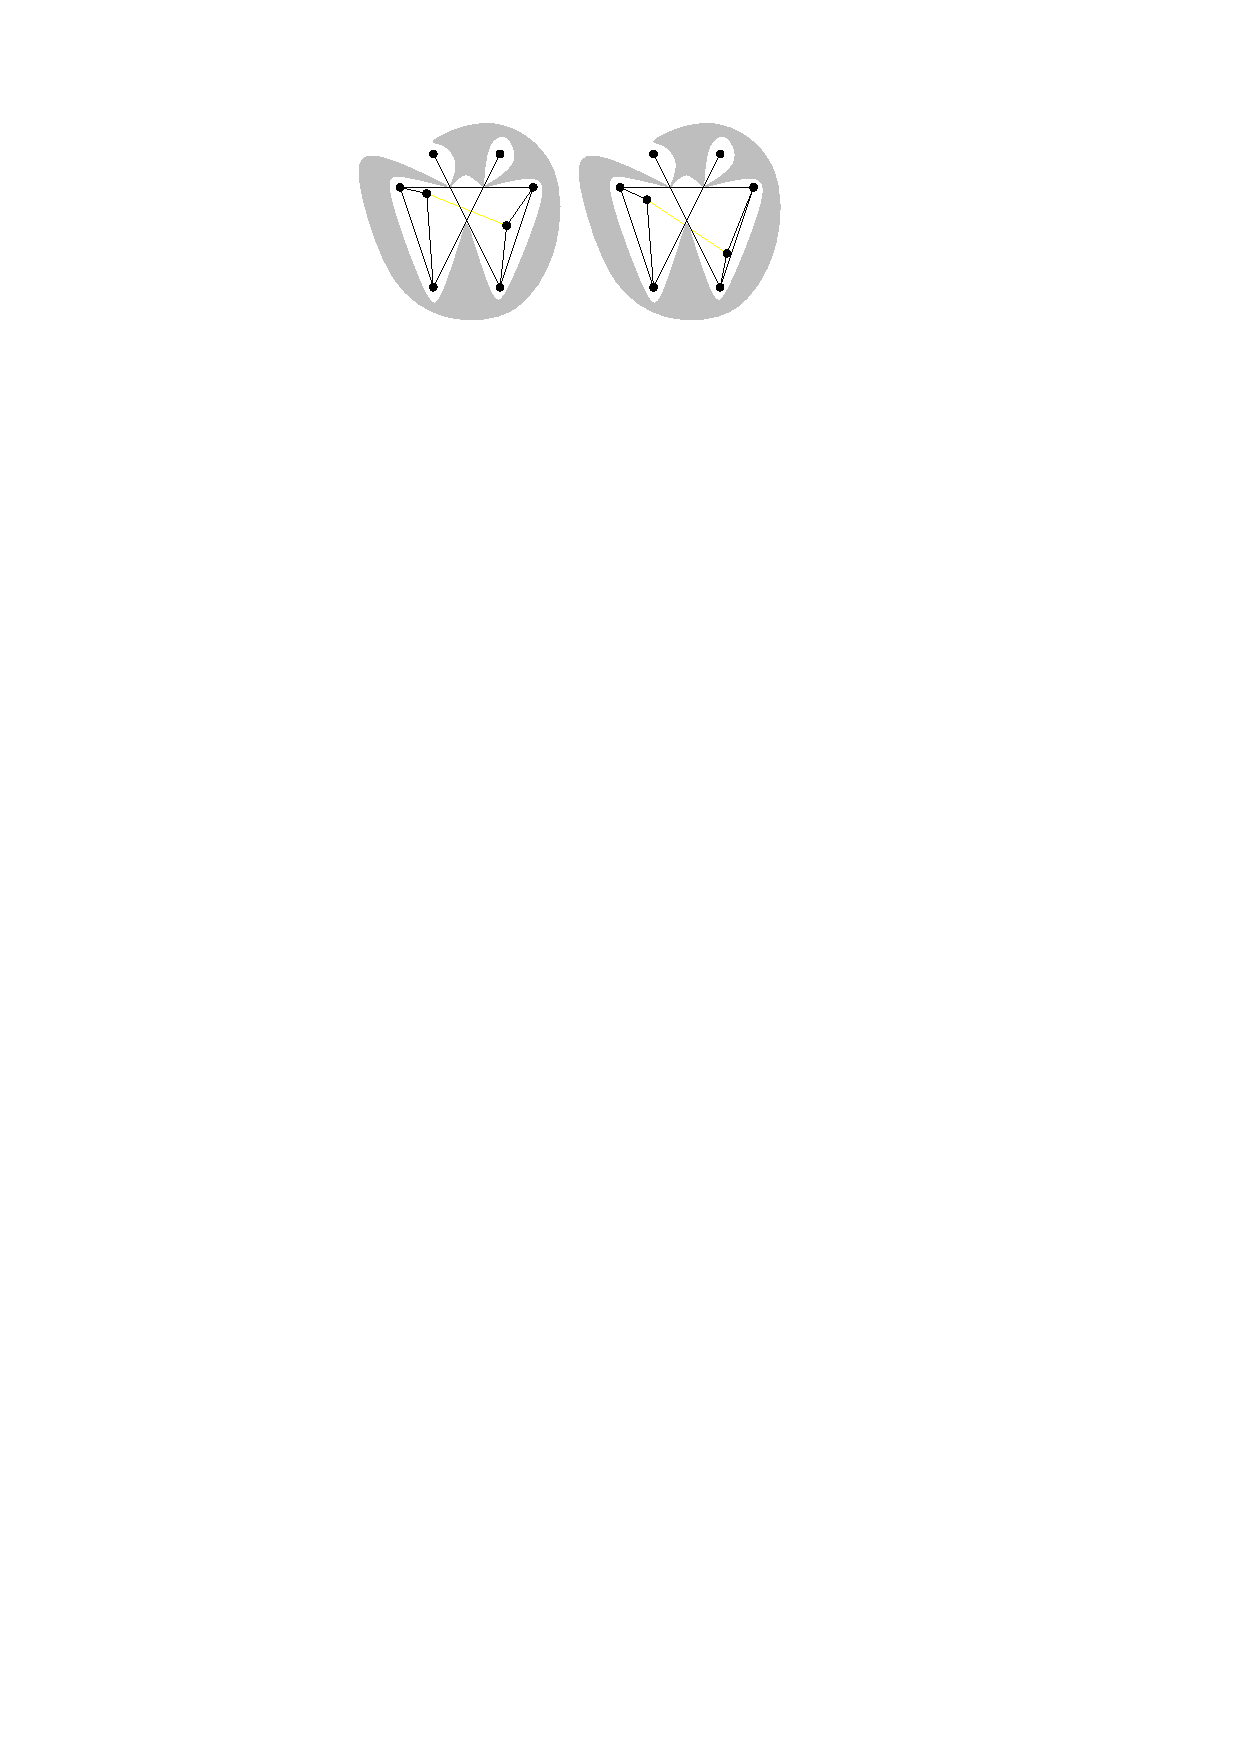
\includegraphics{order-type}
  \end{center}
  \caption{Order type and combinatorial type are insufficient to determine 
      the number of obstacles needed in an obstacle representation.}
  \figlabel{order-type}
\end{figure}

Luckily, the technique used by Goodman and Pollack in proving upper
bounds on the number of order types and combinatorial types generalizes
readily to the type of the equivalence classes we need.

The \emph{super-order type} of a labelled point set
$P=\{x_1,\ldots,x_n\}\subset\R^2$ is the sequence consisting of elements
in $\{+1,0,-1\}$ that determines for each sextuple $a_1,\ldots,a_6\in P$
whether the intersection of the lines $a_3a_4$ and $a_5,a_6$ is to the
left ($-1$), right ($+1$), or on ($0$) the directed line $a_1a_2$.

\begin{lem}
  Let $G$ be a graph with $n$ vertices and let $P_1$ and $P_2$ be two
  point sets each of size $n$ and that have the same super-order type.
  Then, if $G$ has an $h$-obstacle representation $(\varphi_1,S_1)$
  such that $P_1$ is the image of $\varphi_1$, then $G$ also has an
  $h$-obstacle representation $(\varphi_2,S_2)$ such that $P_2$ is the
  image of $\varphi_2$.
\end{lem}


%A \emph{quad} $(a,b,c,d)\in(\R^2)^4$ is a sequence of points such that
%the polygon whose vertices, in counterclockwise order, are $(a,b,c,d)$
%is simple.  The \emph{vertices} of a quad $q=(a,b,c,d)$ are the points
%$a$, $b$, $c$, and $d$ and the \emph{edges} of $q$ are the 6 pairs
%$\{x,y\}\in\binom{\{a,b,c,d\}}{2}$.  When clear from context, we will
%sometimes treat a quad interchangeably with the simple polygon defined
%by its vertices.
%
%NOTE: Degenerate quads (with 3 or 4 collinear points need to be argued
%about differently.  They still work (even better) because, for these,
%it's impossible to have the edges $ab$, $bc$, $cd$, and $da$ without
%having at least one of $ac$ or $bd$.
%
%For a set $P\subset\R^2$, a \emph{quadset} of $P$ is a set
%$Q=\{q_1,\ldots,q_k\}$ of quads whose vertices are points in $P$,
%such that no two quads have a common edge, and such that, for each
%$q_i,q_j\in \binom{Q}{2}$, the polygons determined by $q_i$ and $q_j$
%have disjoint interiors.
%
%\begin{lem}\lemlabel{quadsets}
%  Let $P$ be any set of $n>4$ points in general position.  Then, for
%  each $k\in\{1,\ldots,\lfloor n/3\rfloor\}$, there exists a set of $k^2$
%  quadsets $Q_1,\ldots,Q_{k^2}$ such that
%  \begin{enumerate}
%    \item $|Q_i| \ge n/k$ for each $i\in\{1,\ldots,k^2\}$;
%    \item For any two quads $p,q\in \bigcup_{i=1}^{k^2} Q_i$, $p$ and $q$
%      have no edges in common.
%  \end{enumerate}
%\end{lem}
%
%\begin{proof}[Proof Sketch]
%  Without loss of generality, assume that no two points of $P$ have the
%  same $x$-coordinate and denote the points of $P$ by $p_1,\ldots,p_n$
%  in order of increasing $x$ coordinate.  Observe that we can obtain a
%  quadset of size $\lfloor (n-1)/4\rfloor$ by using the sets
%  \[
%     \{p_1,p_2,p_3,p_4\}, \{p_4,p_5,p_6,p_7\},
%        \ldots,\{p_{n-3},p_{n-2},p_{n-1},p_{n}\}
%  \]
%  and that these can be partitioned into $\approx k/3$ quadsets each of size at
%  least $n/k$.  We call these the \emph{slab quadsets} of $P$.
%
%  For two integers $i$ and $j$, let $P_{i,j}$ denote the subset of $P$
%  given by
%  \[
%    P_{i,j} = \{ p_{ti+j} : t\in \{1,\ldots,\lfloor(n-j)/i\rfloor\} \}
%  \]
%  The set $P_{i,j}$ has size $\lfloor(n-j)/i\rfloor$ and therefore has
%  $\approx k/3i$ slab quadsets.  To obtain the $k^2$ quadsets required
%  by the lemma we take the slab quadsets for the point sets $P_{i,j}$,
%  for sufficiently many values of $i$ that are not multiples of 2
%  or 3.  For each choice of $i$, we use the slab quadsets from $P_{i,j}$
%  for every $j\in\{0,\ldots,i-1\}$.  That is, the values of $i$
%  are taken from the sequence $\langle 1,5,7,11,13,17,\ldots\rangle$
%  of integers congruent to 1 or 5 modulo 6.  Thus, for each $i$, we obtain
%  $\approx k/3$ quadsets.
%
%  All that remains is to show that the quadsets obtained this way satisfy
%  the second property (edge disjointness) required by the lemma.  To see
%  why this property is satisified, define the \emph{rank} of an edge
%  $p_xp_y$ as $|x-y|$.  Next, observe that the quadsets obtained from
%  $P_{i,j}$ only have edges of ranks in $\{i,2i,3i\}$.  This implies
%  that the quads generated from $P_{i',j'}$ for any $i'>i$ do not have
%  any edges in common with the quads generated from $P_{i,j}$, since
%  $\{i,2i,3i\}\cap\{i',2i',3i'\}=\emptyset$ (recall that neither $i$
%  nor $i'$ is a multiple of 2 or 3).
%
%  The only remaining possibility is that the edges of quads obtained
%  from $P_{i,j}$ overlap with the edges of quads obtained from $P_{i,j'}$
%  for some $j'\neq j$.  But this is certainly not possible since the point
%  sets $P_{i,j}$ and $P_{i,j'}$ are disjoint.
%\end{proof}
%
%\begin{lem}
%  Let $G=(V,E)$ be an Erd\"os-Renyi random graph $G_{n,\frac{1}{2}}$,
%  let $P\subset\R^2$ be a set of $n$ points in general position, let
%  $\varphi:V\rightarrow P$ be a bijection between $V$ and $P$ that is
%  independent of the choices of edges in $G$, and let $(\varphi, S)$ be
%  an obstacle representation of $G$ using the minimum number of obstacles
%  (subject to $G$ and $\varphi$).  Then
%  \[
%     \Pr\{|S| < n/128k\} \le e^{-nk/512}
%  \]
%\end{lem}
%
%\begin{proof}
%  Let $Q_1,\ldots,Q_{k^2}$ be the quadsets of $P$ guaranteed by
%  \lemref{quadsets} and let $G'$ be the geometric graph defined by
%  the embedding, $\varphi$, of $G$ onto $P$.  
%
%  We say that a quad, $q=(a,b,c,d)$ \emph{survives} in $G$ if the edges
%  $ab$, $bc$, $cd$, and $da$ are in $G'$ and the edges $ac$ and $bd$ are
%  not in $G'$.  Observe that, in any obstacle representation $(\varphi,S)$
%  of $G$, there must be an obstacle contained in the interior of $q$:
%  Some obstacle, $s$, must intersect the interior of $q$ since, otherwise
%  at least one of the segments $ac$ or $bd$ do not intersect any obstacle;
%  the obstacle $s$ must be contained in the interior $q$, since otherwise
%  at least one of the segments $ab$, $bc$, $cd$, or $da$ intersects $s$.
%
%  Consider some quadset, $Q_i$ and recall that $|Q_i|\ge n/k$.
%  The probability that a particular quad in $Q_i$ survives in $G$ is
%  exactly $1/64$ and, since no two quads share an edge, the number of
%  quads in $Q_i$ that survive is a binomial$(|Q_i|,1/64)$ random variable.
%  Let $\mathcal{E}_i$ denote the event ``less than $n/128k$ quads
%  of $Q_i$ survive in $Q$.''  By Chernoff's Bound on the head of the
%  binomial distribution,
%  \[
%    \Pr\{\mathcal{E}_i\}
%      \le e^{-|Q_i|/512} \le e^{-n/512k} \enspace .
%  \]
%
%  If the event $\mathcal{E}_i$ does not occur then the minimum number of
%  obstacles in $S$ is at last $n/128k$.  Finally, observe that the
%  events $\mathcal{E}_1,\ldots,\mathcal{E}_{k^2}$ are indepedent, since
%  none of the quads in $\bigcup_{i=1}^{k^2} Q_i$ have any edges in common.
%  Therefore
%  \begin{align*}
%    \Pr\{|S|\le (\alpha/128)n/k\} 
%      & \le \Pr\{ \mathcal{E}_1\cap \mathcal{E}_2\cap\cdots\cap\mathcal{E}_{k^2}\} \\
%      & \le \left(e^{-n/512k}\right)^{k^2} \\
%      & = e^{-nk/512} \enspace . \qedhere
%  \end{align*}
%\end{proof}

%\begin{thm}
%  Let $G=(V,E)$ be an Erd\"os-Renyi random graph $G_{n,\frac{1}{2}}$, then
%  \[
%    \Pr\left\{\obs(G) \le \frac{n}{65536(c+5)\ln n}\right\} 
%         \le e^{-cn\ln n + o(cn\ln n)} \enspace .
%  \]
%  In particular, for any sufficiently large constant $c$, this probability
%  is less than one, so there exists graphs having obstacle number
%  $\Omega(n/\log n)$.
%\end{thm}
%
%\begin{proof}
%    The number of distinct order types of sets of $n$ points in the plane
%  is $n^{4n+o(n)}$.  For each such order type the number of mappings of 
%  the points of $G$ onto points of the order type is $n!$.  Therefore, the
%  total number of order type/mapping pairs is at most
%  \[
%    n^{4n+o(n)}n! < n^{5n+o(n)} = e^{5n\ln n+o(n\ln n)} \enspace .
%  \]
%  On the other hand, \lemref{quadsets} states that the probability that
%  any particular order type/mapping pair yields an obstacle representation
%  with fewer than $n/128k$ obstacles is at most
%  \[
%     e^{-kn/512} \enspace .
%  \]
%  Therefore, by the union bound, the probability that there exists any
%  obstacle representation of $G$ using fewer than $n/128k$ obstacles is
%  at most
%  \[
%     e^{5n\ln n+o(n\ln n)-kn/512} .
%  \]
%  Taking $k=512(c+5)n\ln n$ completes proof.
%\end{proof}
%
%NOTE: The constant 65536 can be improved considerably.  By arguing about
%quads a little more carefully and using $G_{n,\frac{4}{5}}$,
%the number of quads becomes a binomial random variable with probability
%$4^4/5^5\approx 1/12$.
%
%NOTE: Using order types in the proof of the preceding theorem is overkill.
%A simpler form of order-type that defines only the orientations important
%for our quadsets could be used instead.  There are only $e^{O(nk)}$ such
%order types.  Unfortunately, this doesn't get us above $\Omega(n/\log
%n)$ because there are still $n!$ ways of embedding the graph onto the
%order type.
%
%NOTE: Pach \etal\ prove their result by showing that the number of
%graphs with obstacle number at most $h$ is at most $2^{O(hn\log^2 n)}$.
%Does our proof improve this bound?
%

\section{Remarks}

Our proof of \thmref{main} relates the problem of counting the number
of $n$-vertex graphs with obstacle number at most $h$ to the problem of
determining the worst-case obstacle number of a graph with $n$ vertices.
Any improvement on the upper-bound for the counting problem will
immediately translate into an improved lower-bound on the worst-case
obstacle number.

\end{document}



